%\section{Evaluation: Scalability of the Current Implementation}\label{sec:evaluation}
\section{Evaluation}\label{sec:evaluation} 
%-------------------------------------------------------------------------------
%Evaluation: How does it really work in practice? Provide real or simulated
%performance metrics, end-user studies, mention external technology adoptors,
%if any, etc.

%This section presents the detailed results you have obtained. If the paper
%is theoretical, you might want to show curves obtained from your equations.
%If the paper is experimental, you will be presenting curves showing the
%measurement results. In order to choose the proper curves to present, you
%must first be clear what point you are trying to convey to the reader. The 
%curves can then be chosen to illustrate this point. Whether your paper is
%theoretical or experimental, you must provide a careful interpretation of
%what your results mean and why they behave as they do.
%-------------------------------------------------------------------------------
% This section presents the detailed results obtained. It contains the results
% obtained from the analytical model, the emulations and the simulations realized
% as well as the interpretation and discussion of them. 
%-------------------------------------------------------------------------------
% The goals of the study,
% The system boundaries
% System services and possible outcomes
% Selected performance metrics
% System and workload parameters
% Factors and their values
% Evaluation techniques
% Selected workload
% Design of the experiments
% Analysis and interpretation of the data
% Presentation of the results
%------------------------------------------------------------------------------_

Evaluation: How does it really work in practice? Provide real or simulated
performance metrics, end-user studies, mention external technology adopters,
if any, and so on.

This section presents the detailed results you have obtained. If the paper
is theoretical, you might want to show curves obtained from your equations.
If the paper is experimental, you will be presenting curves showing the
measurement results. In order to choose the proper curves to present, you
must first be clear what point you are trying to convey to the reader. The 
curves can then be chosen to illustrate this point. Whether your paper is
theoretical or experimental, you must provide a careful interpretation of
what your results mean and why they behave as they do.

See \Cref{fig:example1} and \Cref{fig:example2}.

\begin{figure}
    \centering
    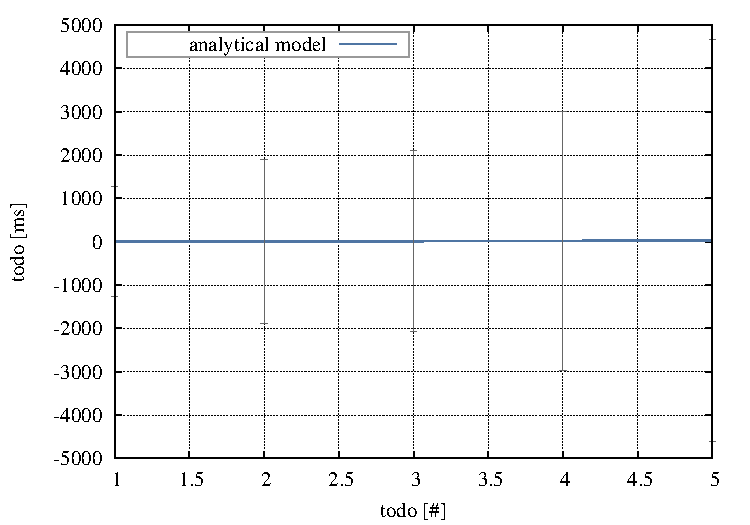
\includegraphics[width=.45\textwidth]{resources/images/example1.pdf} 
    \caption{Example image.}\label{fig:example1}
\end{figure}

\begin{figure}
    \begin{subfigure}[b]{.5\textwidth}
    	\centering
		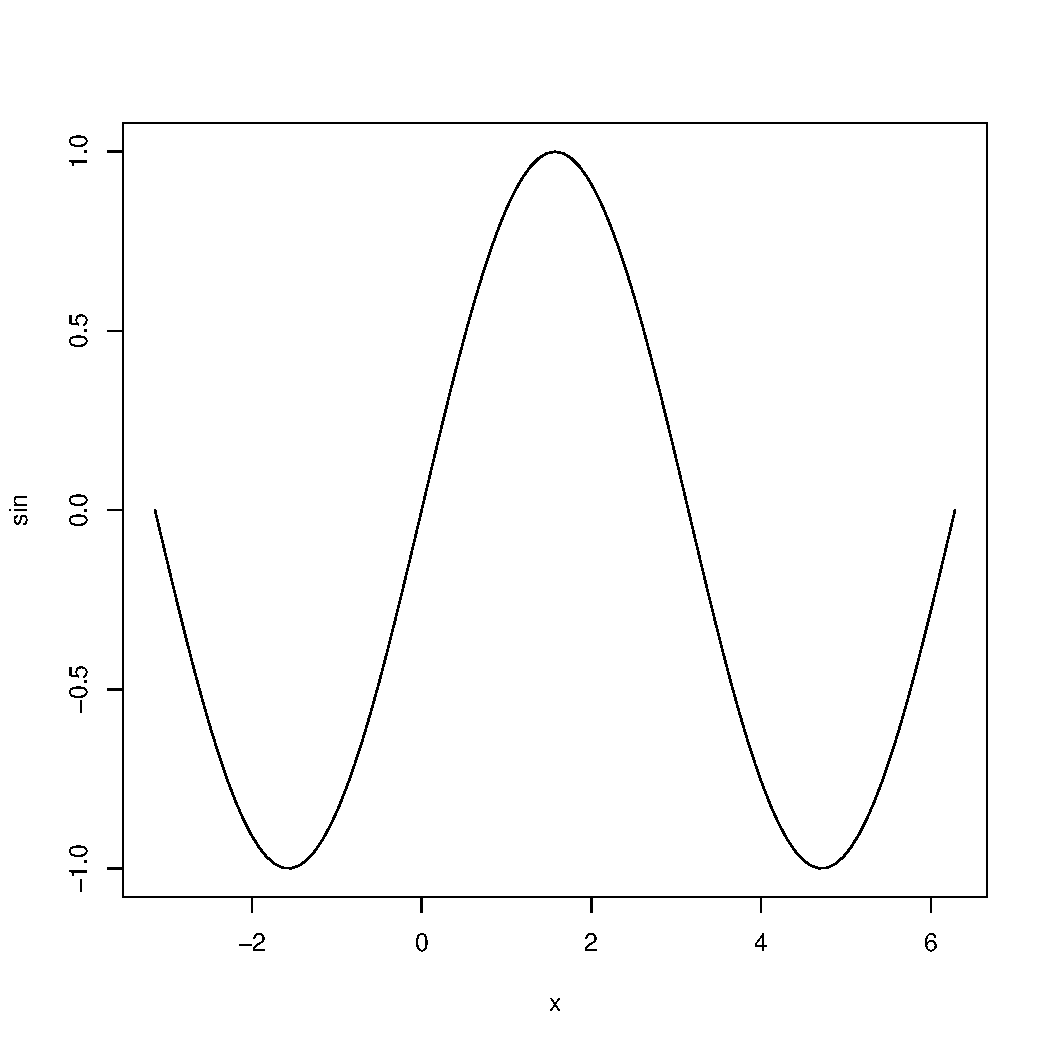
\includegraphics[width=.5\textwidth]{resources/images/example2.pdf}
		\caption{Example2}\label{fig:example2}
    \end{subfigure}
    \begin{subfigure}[b]{.5\textwidth}
    	\centering
		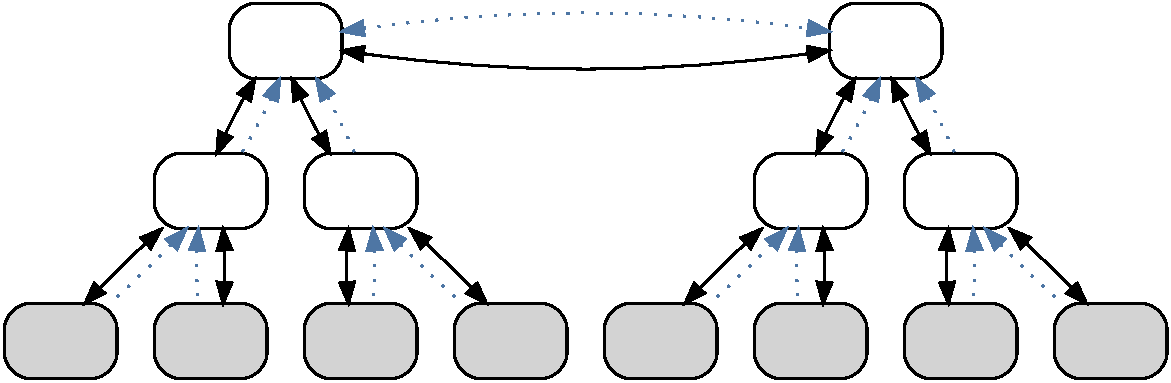
\includegraphics[width=.5\textwidth]{resources/images/example3.pdf}
		\caption{Example3}\label{fig:example3}
    \end{subfigure}    
    \caption{Example images.}\label{fig:exammple2_3}
\end{figure}
